%System Design

\chapter{Implementation}
\label{chapter5_i}
In this chapter we describe the framework and application implementation. We refer to the technologies we used and their interaction. In some cases we cite some crucial code chunks and explain them. Initially, we describe the REST API and we analyze its contents. After an extensive illustration of the back end tier of the framework, we emphasize in the front end, where we mention the used technologies and their implementation. Alongside the front end description, we present some fragments of front end use cases.

\section{General JavaScript practices and patterns}
\begin{figure}
	\centerline{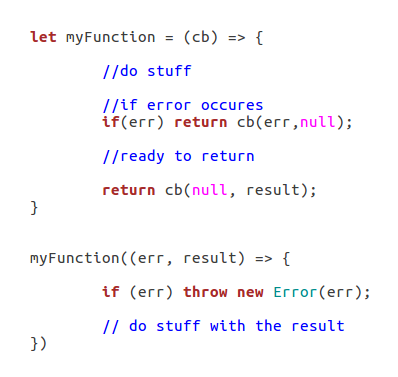
\includegraphics[scale=0.7]{cb.png}}
	\caption{Example of a callback function}
	\label{cb}
\end{figure} 
In the framework we developed, we make use of javascript in both front and back end. This programming language uses asynchronous logic, which takes place through the usage of asynchronous callback functions. A callback function is a method which receives as an argument another method, in order to call it later. The execution of the first function does not block the execution of the rest of the program commands. The execution of the callback function begins, when the execution of the first function is completed. An example of a callback function can be seen in figure ~\ref{cb}. \par
	In our framework, the callback functions are used constantly, so that the design and implementation are transformed accordingly. As a convention, all the callback functions receive as arguments two objects, the error and the result object. Before the execution of the callback function, in case an error occurs, the execution stops and the error object is passed to the callback. The result object is obviously null. If no errors occur, the error object is null and the result object contains the function outcome. Following we describe two design patterns, which are based in callback functions and are heavily used in the framework implementation.

\subsection{Closures}
\begin{figure}
	\centerline{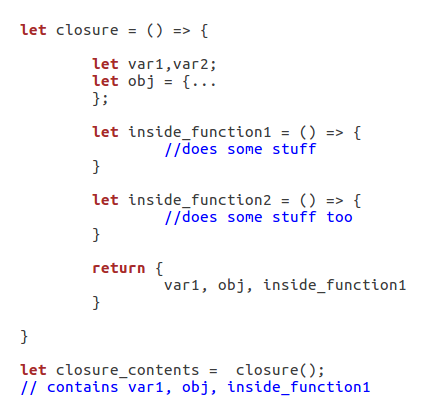
\includegraphics[scale=0.7]{closure.png}}
	\caption{Example of a closure function}
	\label{closure}
\end{figure} 
Javascript is an object oriented language and was created to perform well in any platform. Thus, it has many ways of defining certain structures, such as classes. In our framework, we define our classes through the closure design pattern. Closures fully implement a class functionality.\par
	Generally, a closure in javascript is a function. This function receives arguments that initialize its state. The function body defines contents, such as variables, objects and other functions. Finally, the function returns, or exposes in the rest of the framework, only what is necessary. This may include also variables, objects and functions. Anything that is not returned, equals to what classes define as private. An example of this pattern is shown in figure ~\ref{closure}.

\subsection{Thunks}
\begin{figure}
	\centerline{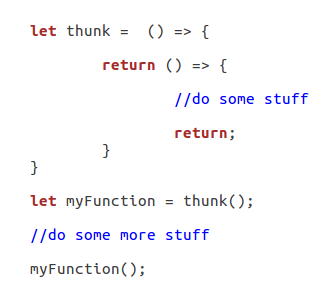
\includegraphics[scale=0.7]{thunk.png}}
	\caption{Example of a thunk function}
	\label{thunk}
\end{figure} 
The thunk pattern has a similar structure with closure, but it's used in a different way. Basically, it's a function which returns another function. The interesting part is that the execution of the first function does not imply the execution of the second. In this way we define "lazy" functions, that is methods which are scheduled to execute but don't until they have to. This pattern is important for solving a problem that occurs in javascript, known as callback hell. This problem is caused by the generation of large sequences of nested callback functions, which is considered a bad design practice and creates debug problems. An example of the thunk pattern is shown in figure ~\ref{thunk}.

\section{Back End implementation}
In this section we focus in the back end implementation of the framework. Initially we present the REST API and then we describe the development stages of the framework modules. We emphasize in the technologies used and their in between communication (interoperability).

\subsection{REST API}
An important part of the back end framework implementation is the development of the REST API, which is achieved through routing. Routing refers to determining how an application responds to a client request for a specific endpoint, which is a URI (or path) and a specific HTTP request method (GET, POST, PUT or DELETE). Each of our routes has different handler functions which are executed when the route is matched. The route handler functions use the information which is given to them through the request, and after the execution of internal operations, return a response object to the client.\par
	 The response object has a concrete structure and includes all the required information. Among other things, it contains the status code and the result data. Generally the content of the response object is determined by the request method and the success of the operation (error handling is described thoroughly in chapter ~\ref{errorHandling}). The structure of the response object implements the JSON format. \par 
	 	Following we present all the routes for each model entity seperately. For some of them we describe their corresponding handlers.
	 	
\paragraph{}
\begin{table}[]
\centering
\begin{tabular}{|c|c|}
\hline
\rowcolor[HTML]{32CB00} 
\textbf{URI}     & \textbf{method} \\ \hline
\rowcolor[HTML]{FFFFFF} 
/login           & GET             \\ \hline
\rowcolor[HTML]{67FD9A} 
/logout          & GET             \\ \hline
\rowcolor[HTML]{FFFFFF} 
/isauthenticated & GET             \\ \hline
\end{tabular}
\caption{Authentication URI's}
\label{authURI}
\end{table}
The routes of the table ~\ref{authURI} are used by the framework for the authentication of the users. The login route checks whether the client's credentials exist in an instance of the users model of the database. If the client is identified, a positive confirmation is sent to the user, while at the same time a session cookie is saved (session management is described in chapter ~\ref{security}). Otherwise, the server's response is negative. The logout route disconnects the user from the framework and its corresponding session cookie is deleted from the database. The last route is used from the framework to check if the user is already authenticated. If this event occurs, the authentication step is skipped.

\paragraph{Users}
\begin{figure}
	\centerline{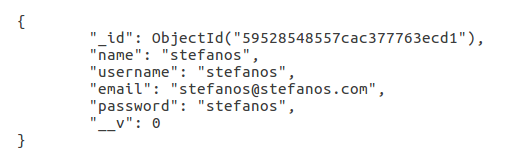
\includegraphics[scale=0.7]{userObject.png}}
	\caption{Example of a User instance}
	\label{userObject}
\end{figure}
\begin{table}[]
\centering
\begin{tabular}{|c|c|c|}
\hline
\rowcolor[HTML]{32CB00} 
\textbf{Model} & \textbf{URI}                                                     & \textbf{method}                                     \\ \hline
\rowcolor[HTML]{FFFFFF} 
Users          & /users/?id=\{user\_id\}                                              & GET                                                 \\ \hline
\rowcolor[HTML]{67FD9A} 
Users          & /register                                                        & POST                                                \\ \hline
\rowcolor[HTML]{FFFFFF} 
Users          & /users/?id=\{user\_id\}                                              & PUT                                                 \\ \hline
\rowcolor[HTML]{67FD9A} 
Users          & \multicolumn{1}{l|}{\cellcolor[HTML]{67FD9A}/users/?id=\{user\_id\}} & \multicolumn{1}{l|}{\cellcolor[HTML]{67FD9A}DELETE} \\ \hline
\end{tabular}
\caption{Users URI's}
\label{usersURI}
\end{table}
Table ~\ref{usersURI} presents the routes which concern the users model. The POST method is responsible for the creation of new user instances. It checks whether all fields have a value and, the username and email properties are unique. The figure ~\ref{userObject} presents the structure of a User instance. The GET method returns the user instance information and the projects in which he participates. The PUT and DELETE methods are used for their corresponding functionalities.

\paragraph{Projects}
\begin{figure}
	\centerline{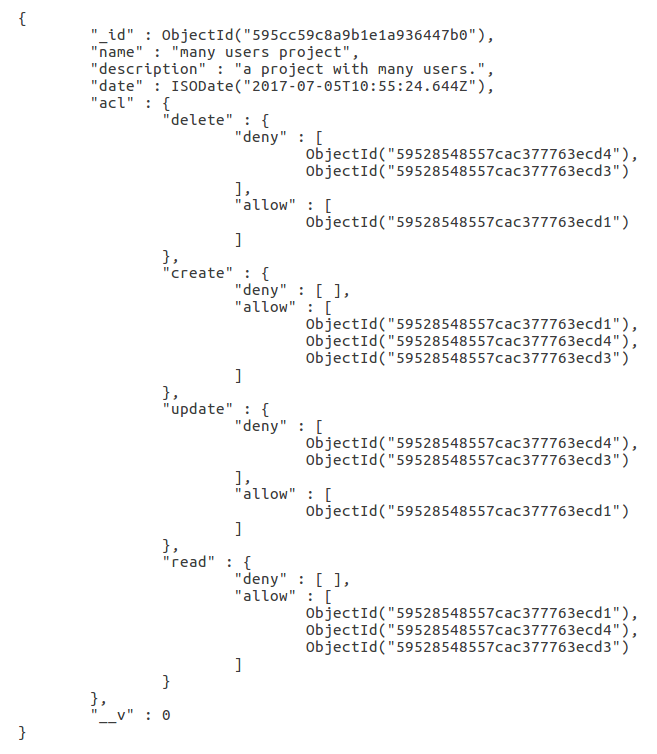
\includegraphics[scale=0.7]{projectObject.png}}
	\caption{Example of a Project instance with three users}
	\label{projectObject}
\end{figure}
\begin{table}[]
\centering
\begin{tabular}{|c|c|c|}
\hline
\rowcolor[HTML]{32CB00} 
\textbf{Model} & \textbf{URI}                   & \textbf{method} \\ \hline
\rowcolor[HTML]{FFFFFF} 
Projects       & /projects/?id=\{project\_id\}      & GET             \\ \hline
\rowcolor[HTML]{67FD9A} 
Projects       & /projects                      & POST            \\ \hline
\rowcolor[HTML]{FFFFFF} 
Projects       & /projects/join/?id=\{project\_id\} & GET             \\ \hline
\end{tabular}
\caption{Projects URI's}
\label{projectsURI}
\end{table}
The Project model REST API is presented in table ~\ref{projectsURI}. The POST method is used for the creation of project model instances. The  figure ~\ref{projectObject} presents the structure of a Project instance. The GET method searches out for a specific project and its elements. Then the datasets and posts which are related to the projects, are returned along with the project information. The join route is responsible for the addition of project members. In order to implement it, an update of the ACL property of the project instance takes place.

\paragraph{Datasets}
\begin{table}[]
\centering
\begin{tabular}{|c|c|c|}
\hline
\rowcolor[HTML]{32CB00} 
\textbf{Model}                                         & \textbf{URI}                                                               & \textbf{method}                                     \\ \hline
\rowcolor[HTML]{FFFFFF} 
Datasets                                               & /datasets/?id=\{dataset\_id\}                                              & GET                                                 \\ \hline
\rowcolor[HTML]{67FD9A} 
Datasets                                               & /datasets                                                                  & POST                                                \\ \hline
\rowcolor[HTML]{FFFFFF} 
Datasets                                               & /datasets/list/?id=\{dataset\_id\}                                         & GET                                                 \\ \hline
\rowcolor[HTML]{67FD9A} 
Datasets                                               & /datasets/grid/?id=\{dataset\_id\}                                         & GET                                                 \\ \hline
\rowcolor[HTML]{FFFFFF} 
\multicolumn{1}{|l|}{\cellcolor[HTML]{FFFFFF}Datasets} & \multicolumn{1}{l|}{\cellcolor[HTML]{FFFFFF}/datasets/?id=\{dataset\_id\}} & \multicolumn{1}{l|}{\cellcolor[HTML]{FFFFFF}DELETE} \\ \hline
\end{tabular}
\caption{Datasets URI's}
\label{datasetsURI}
\end{table}
The routes of the table ~\ref{datasetsURI} are developed for the Datasets model. A general analysis of the dataset save and retrieval management is described in chapter ~\ref{pyfiles}. The GET method returns the contents of an HDF file. The POST and DELETE methods are responsible for the creation and deletion of a dataset, respectively. The list route returns a list of datasets, which are contained in a project. Also, the grid route returns a chunk of an array, which is located inside a dataset, in order to present it to the client.

\paragraph{Posts}
\begin{table}[]
\centering
\begin{tabular}{|c|c|c|}
\hline
\rowcolor[HTML]{32CB00} 
\textbf{Model} & \textbf{URI}            & \textbf{method} \\ \hline
\rowcolor[HTML]{FFFFFF} 
Posts          & /posts/?id=\{post\_id\} & GET             \\ \hline
\rowcolor[HTML]{67FD9A} 
Posts          & /posts                  & POST            \\ \hline
\rowcolor[HTML]{FFFFFF} 
Posts          & /posts/?id=\{post\_id\} & UPDATE          \\ \hline
\rowcolor[HTML]{67FD9A} 
Posts          & /posts/?id=\{post\_id\} & DELETE          \\ \hline
\end{tabular}
\caption{Posts URI's}
\label{postsURI}
\end{table}
\begin{figure}
	\centerline{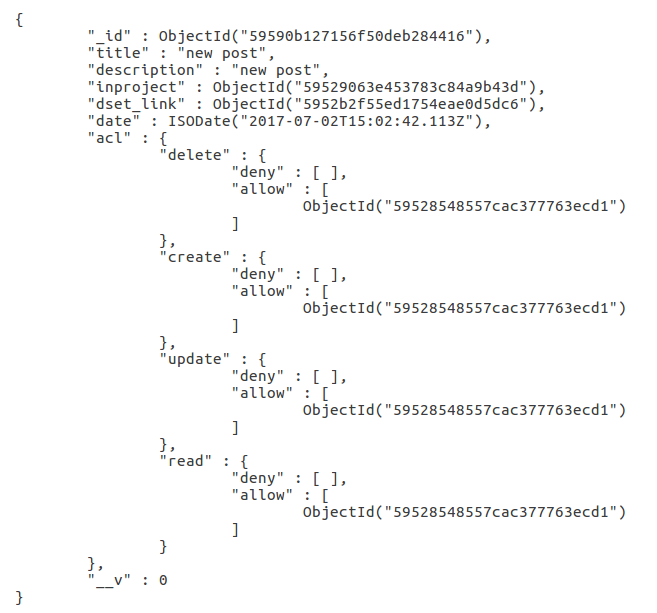
\includegraphics[scale=0.7]{postObject.png}}
	\caption{Example of a Post instance}
	\label{postObject}
\end{figure}
Table ~\ref{postsURI} presents the routes which are related to the posts model. All the methods are used for the corresponding functionalities. The figure ~\ref{postObject} presents the structure of a Post instance. 

\paragraph{Plots}
\begin{table}[]
\centering
\begin{tabular}{|c|c|c|}
\hline
\rowcolor[HTML]{32CB00} 
\textbf{Model} & \textbf{URI}            & \textbf{method} \\ \hline
\rowcolor[HTML]{FFFFFF} 
Plots          & /plots/?id=\{plot\_id\} & GET             \\ \hline
\rowcolor[HTML]{67FD9A} 
Plots          & /plots                  & POST            \\ \hline
\rowcolor[HTML]{FFFFFF} 
Plots          & /plots/?id=\{plot\_id\} & DELETE          \\ \hline
\end{tabular}
\caption{Plots URI's}
\label{plotsURI}
\end{table}
\begin{figure}
	\centerline{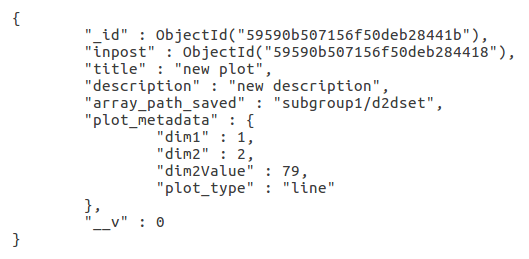
\includegraphics[scale=0.7]{plotObject.png}}
	\caption{Example of a Plot instance}
	\label{plotObject}
\end{figure}
The Plot model REST API is presented in table ~\ref{plotsURI}. All the methods are used for the corresponding functionalities. The figure ~\ref{plotObject} presents the structure of a Plot instance. 


\subsection{NoSQL Access Management}
In chapter ~\ref{nosql} a thorough description of the design of the noSQL access module is presented. In this chapter we mention the technologies we used and the implementation of this module. \par
	A standard library we use in this module is Mongoose.js. This library offers  a schema based solution in the modelling of the database for node.js. It grants complete CRUD operations which we use in data access object module. These operations are developed as callback functions, so the execution of the function does not stop the code flow. When the execution of a CRUD operation is completed, a callback function is called. Also, the data communication between the internal modules and the mongoose library is implemented through javascript objects.

\subsection{Security Management}
\label{security}
In chapter ~\ref{def} we present the general idea of the security design. Here we describe how these modules are combined to implement the security objective. The technologies we use are presented too. Initially, we introduce the passport javascript module, which has the key role in session management. \par
	Passport is a node.js library which is used for the user authentication. When a user logs in the framework, the library creates a cookie object which is saved in a database collection. Furthermore, it embodies this cookie in the respond object, which is sent to the client. This operation is called serialization. The client saves the cookie object and sends it back to the future requests. When the user logs out or a certain amount of time has passed without connecting to the system, the passport library deletes the user cookie from the database. This operation is called deserialization. The framework ensures the correct communication between the login- logout routes and their corresponding handlers, the passport library and the database collection. \par 
	The defender middleware module combines the authentication/session management functionality we described above, with the authorization functions that are introduced in the noSQL access module. Initially, the system investigates if the request object includes the required cookie, so that the authentication can be completed. If the operation succeeds, the request object URI is examined. With some exceptions, the URI's first part corresponds to one of the models  the database provides. Also, the request method must be one of GET, POST, UPDATE or DELETE. \par 
	The last part of the security module is the authorization investigation of the framework. As mentioned in chapter \ref{nosql}, the functionality of the permissions model includes functions which investigate permissions of a model instance. At this point we use isAllowed and isAllowedCreate functions to check if the request is allowed to proceed. If the examination is successful, the middleware operation is completed and the routes module is called. In all situations that the check fails, the access is denied for the user and a corresponding status code is returned (401 if not authenticated and 403 if not authorized).

\subsection{Python - Node.js Interoperability}
As aforementioned in chapter ~\ref{hdf}, HDF is an essential ingredient of the framework for storing multidimensional datasets. The HDF library is developed in C/C++, which constitutes it as foreign code to our framework. Firstly we studied ways of embedding foreign code in node.js. An option for establishing inter-processing communication (IPC) is over Standard Input/Output (STDIO), available in all major operating systems.\par 
	Although an opensource project which exposes the HDF functionality directly to node.js exists, we observed prohibitive inefficiencies in its implementation. Thus, we set upon a more mature python implementation, the h5py. A module responsible for sending messages from our framework to h5py, and inversely, was developed. The rest of this section is dedicated to the way this module operates.\par 
	Node.js includes a spawn functionality of the child process module, which allows invocation of external processes, parameterized by arguments. The results of the python execution are manipulated by the event listener, returned by the child process. The controller listens for the data and error events. In case of an error, a new error object is propagated, while in the opposite case the result is parsed. \par 
	We use the included python's JSON library, which enables easy information parsing to a javascript object. Via the STDOUT buffer, all the results are serialized and accessed from javascript. We design a communication protocol between python and node.js, for the customization of the script functions. Python executes the corresponding commands, returning successful results or potential errors.


\section{Front-End Implementation}
In this section we continue with the description of the front end part of the implementation. While initially we investigated different framework options for the client tier, we ended up using pure javascript. We considered overkill the usage of a large framework for our requirements. This way we pursued the better understanding of javascript's front end functionality. In addition, it is important to point out that the lack of context switching aids productivity, when using javascript end to end. We were satisfied with the usage of small libraries, whenever it was necessary. \par 
	A fundamental characteristic of our framework's front end is the single page application design approach, as explained in chapter ~\ref{spa}. According to this architecture, all the essential code is retrieved in the front end in a single page load. Then, the communication between client and server is based entirely in ajax requests (see chapter~\ref{ajax}). In order to implement this approach, we used a library called browserify. This library offers the ability to require files, as node.js uses it. Then it scans and finds all the files which use the require functionality and bundles them in one file, so it can be sent to the client. \par
	This functionality solves many of our problems. Firstly, it's not vital anymore to write all the files inside script tags in the html files one by one, based on the dependency and execution order. But the great advantage is that a corresponding model of the back end is implemented in the front end part of the framework. Thus, a model hierarchy, which includes modules that can be combined and reused, is defined. In this way, a model driven software development design approach is adopted by the client.

\subsection{Code organization and content}
\begin{figure}
	\centerline{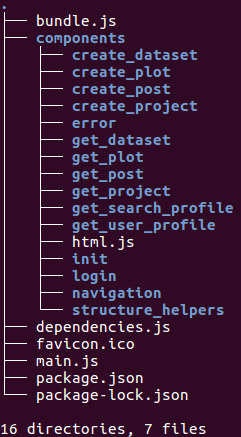
\includegraphics[scale=0.7]{clienttree.png}}
	\caption{Client structure tree}
	\label{clienttree}
\end{figure}
Figure ~\ref{clienttree} represents the general internal structure of the client files. The front end makes use of an approach corresponding to the server and the node.js implementation through the utilization of the node package manager. The package.json file contains vital information for the client network, such as library dependencies, different environment execution scripts etc. The main.js file is the first file to execute, by starting the client's initialization. \par 
\begin{figure}
	\centerline{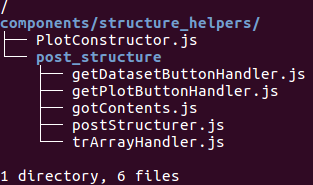
\includegraphics[scale=0.7]{poststructuretree.png}}
	\caption{Post component structure tree example}
	\label{poststructuretree}
\end{figure}
	The components folder includes, among others, all the modules which are executed according to the corresponding user choices. Figure ~\ref{poststructuretree} represents one of these components. It contains submodules responsible for the creation of the appropriate elements. Event handlers modules are also included, in order to manage the functionality of elements, e.g a button. Finally, the component utilizes a module, the purpose of which is the exchange of information between server and client, established via ajax requests.\par
	The communication between the components is secured through the dependencies.js file. This file is received as a parameter in all the components of the client, in order to become available in any case. When the service of a component is terminated, the user interface's content is removed in order to execute another component, which is available through the dependencies.js file.

\paragraph{html.js}
This file is developed to define the front end basic operations, which are related to the html functionality. Starting from core javascript methods, such as createElement or addEventListener, we developed a wrapper adapted to our purpose. The functions create, mountTo and addListenerTo are exposed from this file to the front end and are used constantly in all components. 

\subsection{Plot generation with c3.js}
Plot generation is an essential service of the developed application. In combination with the HDF functionality in the back end, we created a service, through which the users upload their datasets and can visualize them with plots. C3.js is a javascript library, wrapper of D3.js - the core of data visualization tools. This library offers the ability to create simple and minimal diagrams, and supports all simple plot types. \par 
	In order to generate a plot, the arithmetic data must be received and the corresponding configuration must be implemented. The client receives the arithmetic data and the matching metadata in JSON format. After those are parsed, the arithmetic data are prepared for plotting, via the C3 library. The metadata contain useful information, such as the plot type, by means of which we may present our data. \par 
	This library allows us to update the visual plot, which is incredibly useful in front end time saving. Thus, even before the data are received by the client, the corresponding plot presenting process has already started with empty data input. When the data arrive, the plot updates and it is not necessary to create it again. In addition, this logic offers a more smooth experience for the user.
	
\section{Specific framework operations}
In this section we present some parts of the framework which combine the usage of both front and back end.

\subsection{Plot presentation - Zoom functionality}
\begin{figure}
	\centerline{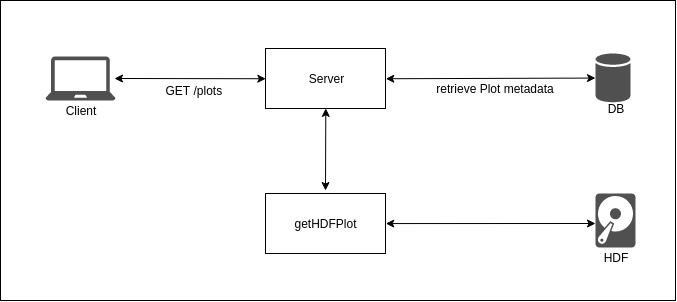
\includegraphics[scale=0.7]{zoom.png}}
	\caption{Plot presentation mechanism}
	\label{zoom}
\end{figure}
In chapter ~\ref{pyfiles} we presented the python scripts which are responsible for the HDF dataset retrieval in JSON format. But how does the plot presentation and zoom functionality operate?\par 
	Figure ~\ref{zoom} presents the actions that must be made inside the framework in order to show a plot to the user. Initially, the user requests the plot display. The front end sends a request, which contains the GET method and the /plot URI, to the corresponding route, along with the specific plot ID. After it is received, the server searches the database for the plot instance and retrieves the related metadata. Following, node.js spawns a new process which executes the getHDFPlot script. This script fetches the HDF file, which contains the plot data, and returns these data in JSON format. Finally, the server is ready to send the result to the client. \par 
	
\begin{figure}
\centering
\begin{subfigure}{1\textwidth}
  \centering
  \centerline{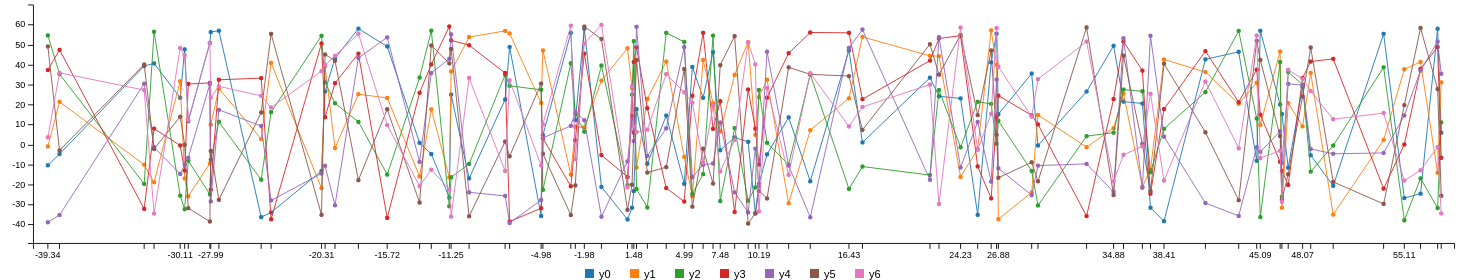
\includegraphics[width=1.2\linewidth]{plotcontentsNOzoom.png}}
  \caption{A plot without zoom}
  \label{fig:sub1}
\end{subfigure}
\begin{subfigure}{1\textwidth}
  \centering
  \centerline{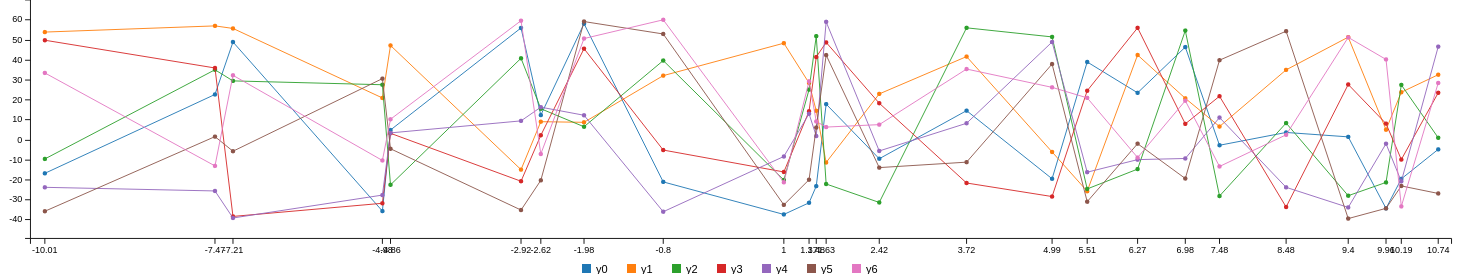
\includegraphics[width=1.2\linewidth]{plotcontentsWITHzoom.png}}
  \caption{A plot with zoom}
  \label{fig:sub2}
\end{subfigure}
\caption{A plot before and after the zoom}
\label{fig:test}
\end{figure}

	To activate the zoom functionality, the user may use the drag and drop mouse technique, to select the first and last point in which he focuses. The corresponding values are sent along the next request as parameters to the server. The procedure is repeated  under the condition that the sampling frequency is calculated based on the parameters distance. The plot which is presented to the user is focused in these specific points.	Figure ~\ref{fig:test} presents the user interface result before and after the zoom.
	
\subsection{Upload functionality}
\begin{figure}
	\centerline{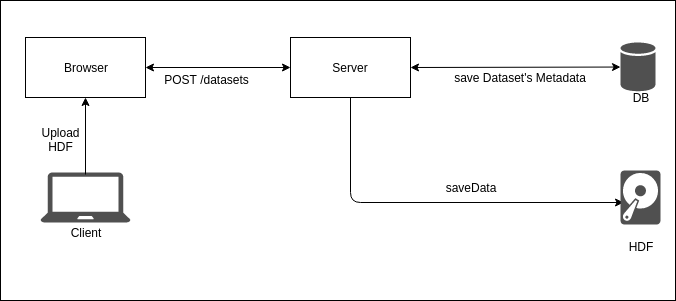
\includegraphics[scale=0.7]{upload.png}}
	\caption{Upload mechanism}
	\label{upload}
\end{figure}
Figure ~\ref{upload} shows the procedure of uploading an HDF file to the framework. Firstly, the file uploads in the browser. Then, the file along with its metadata is sent to the server with a POST method, possibly in chunks of data.  Next, the server checks for the file content, and then saves the HDF file in the filesystem, as explained in chapter~\ref{helpers}. Finally, the file metadata with the unique new filename are saved as a Dataset instance inside the database.

\subsection{Error Handling}
\label{errorHandling}
A very important aspect of the framework is the way through which the system handles its errors. In general, exceptions ~\cite{carlson2000method} are divided in two major categories: those that are created by the client's wrong behaviour, and those that occur from poor software design, also known as bugs. The process by means of which the framework is managing its errors or exceptions of the system, is called error or exception handling. In a framework environment a developer must foresee all the possible exceptions that may occur and provide a handling solution for all of them. The framework must be designed accordingly, by creating a general way of exception handling. \par
	We designed the framework in a way that the handling of an exception happens in the regular flow of the code execution, and not inside a callback function. It is a bad practice to handle the error inside a callback function because the stack trace is lost. We handle the exceptions that occur in the routes and defender modules. All errors are sent with the corresponding status code to the front end. \par 
	 Each time a request to the server is sent by the client, an error check is executed in the response object, in order to handle possible errors. During this check, a potential error is categorized based on the status code, and handled accordingly. In most cases a flash message shows up, but in case of a server error, the error page is presented. \par 
	We pursued the minimization of the number of possible exceptions which occur from the client's wrong behaviour. In order to achieve that, we added in the front end specific conditions, validation restrictions etc, so that it becomes difficult to occur. Also, we implemented a similar logic in the back-end.


\section{Application Presentation}
In this section we briefly present the demo application we created via our framework. Below we show some aspects of the application.

\begin{figure}
\centerline
{
\begin{subfigure}{0.7\textwidth}
  \centering
  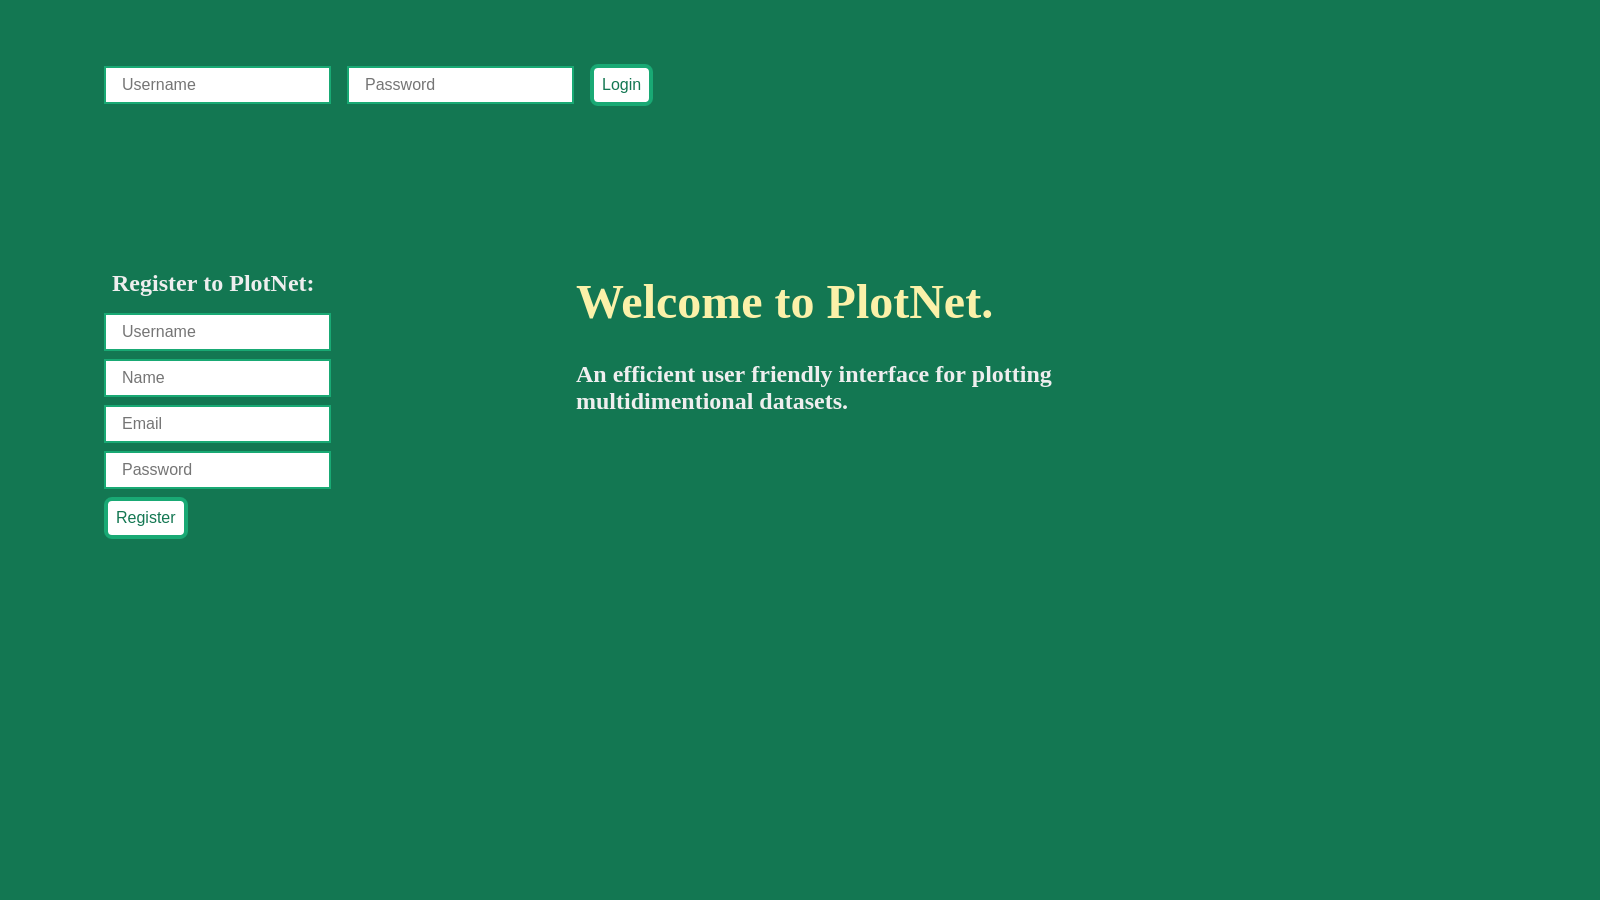
\includegraphics[width=.9\linewidth]{login.png}
  \caption{Login page}
\end{subfigure}%
\begin{subfigure}{0.7\textwidth}
  \centering
  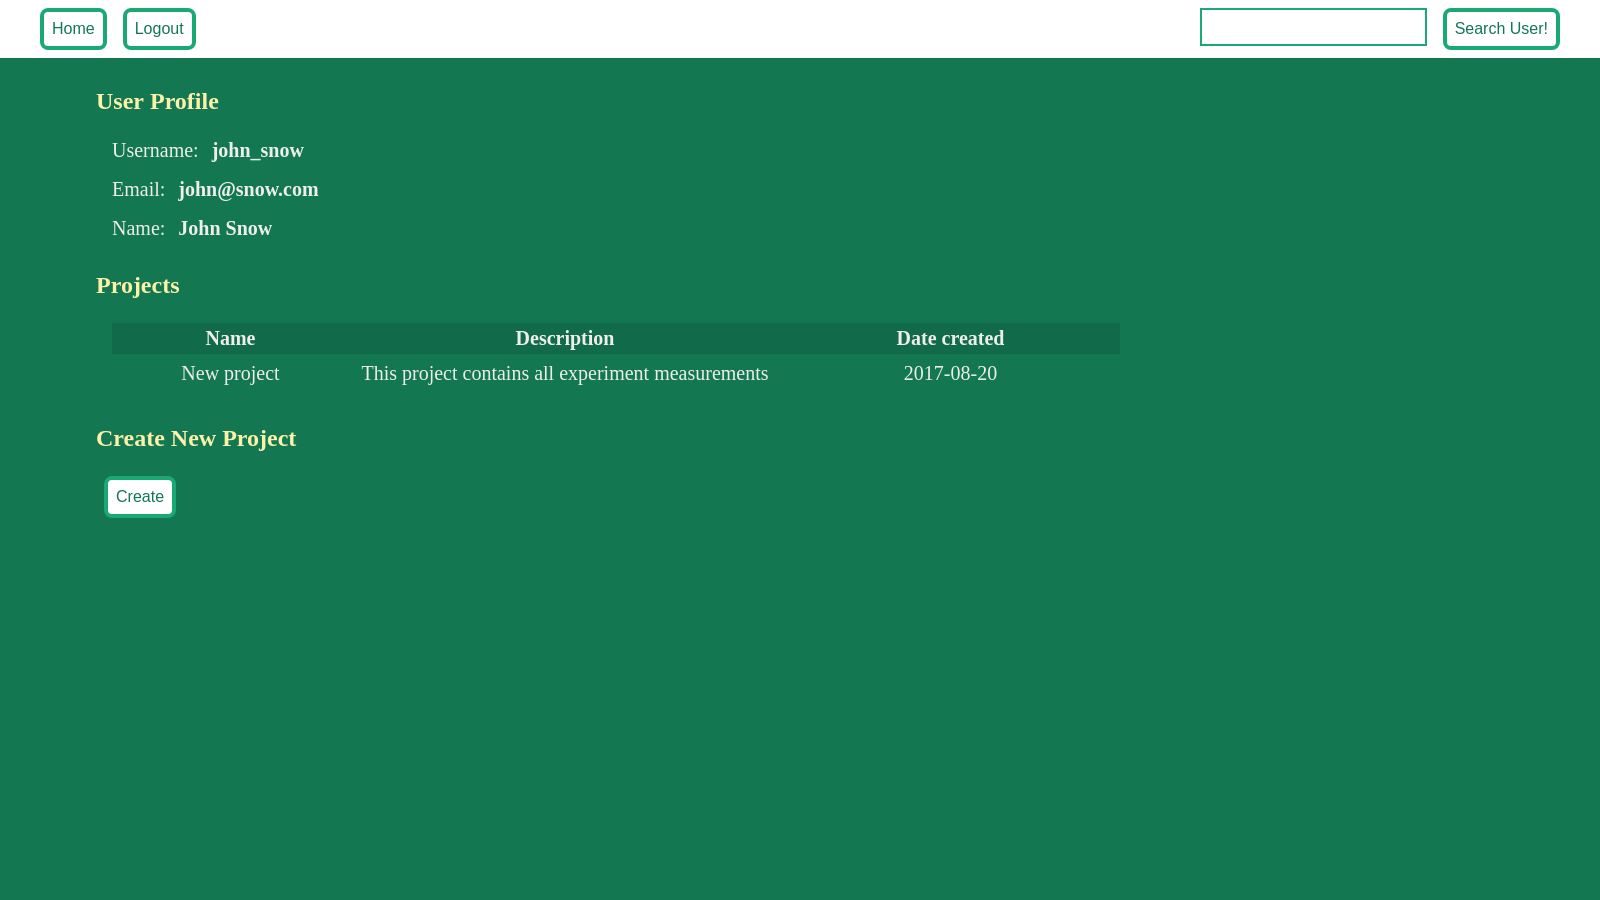
\includegraphics[width=.9\linewidth]{home.png}
  \caption{User home page}
\end{subfigure}}
\centerline
{
\begin{subfigure}{0.7\textwidth}
  \centering
  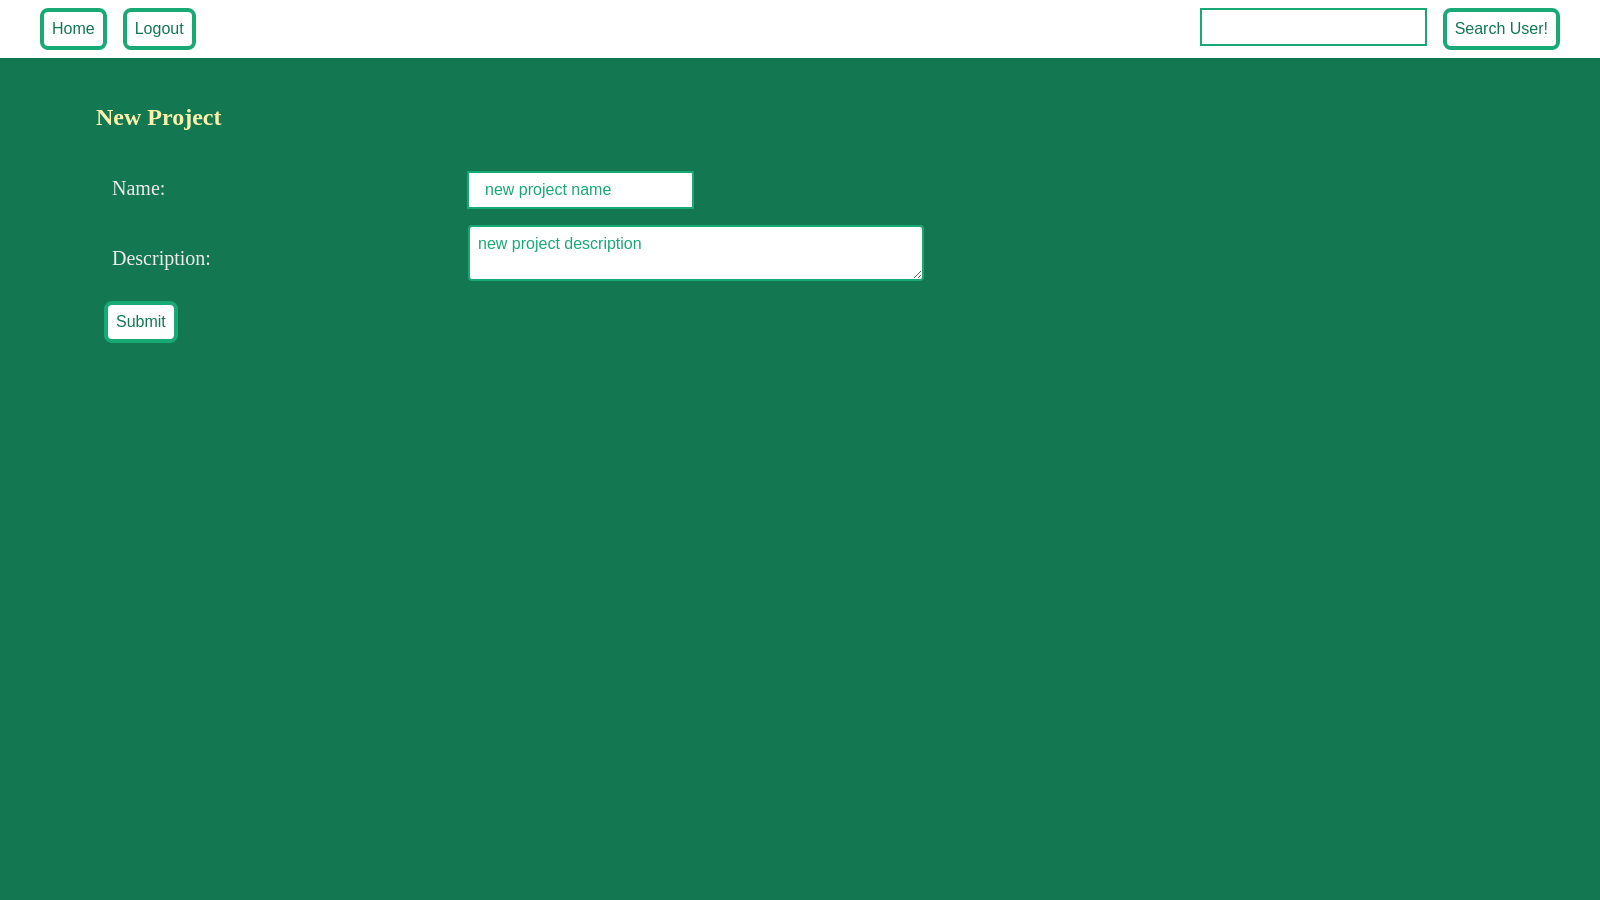
\includegraphics[width=.9\linewidth]{newproject.png}
  \caption{Create new project page}
\end{subfigure}%
\begin{subfigure}{0.7\textwidth}
  \centering
  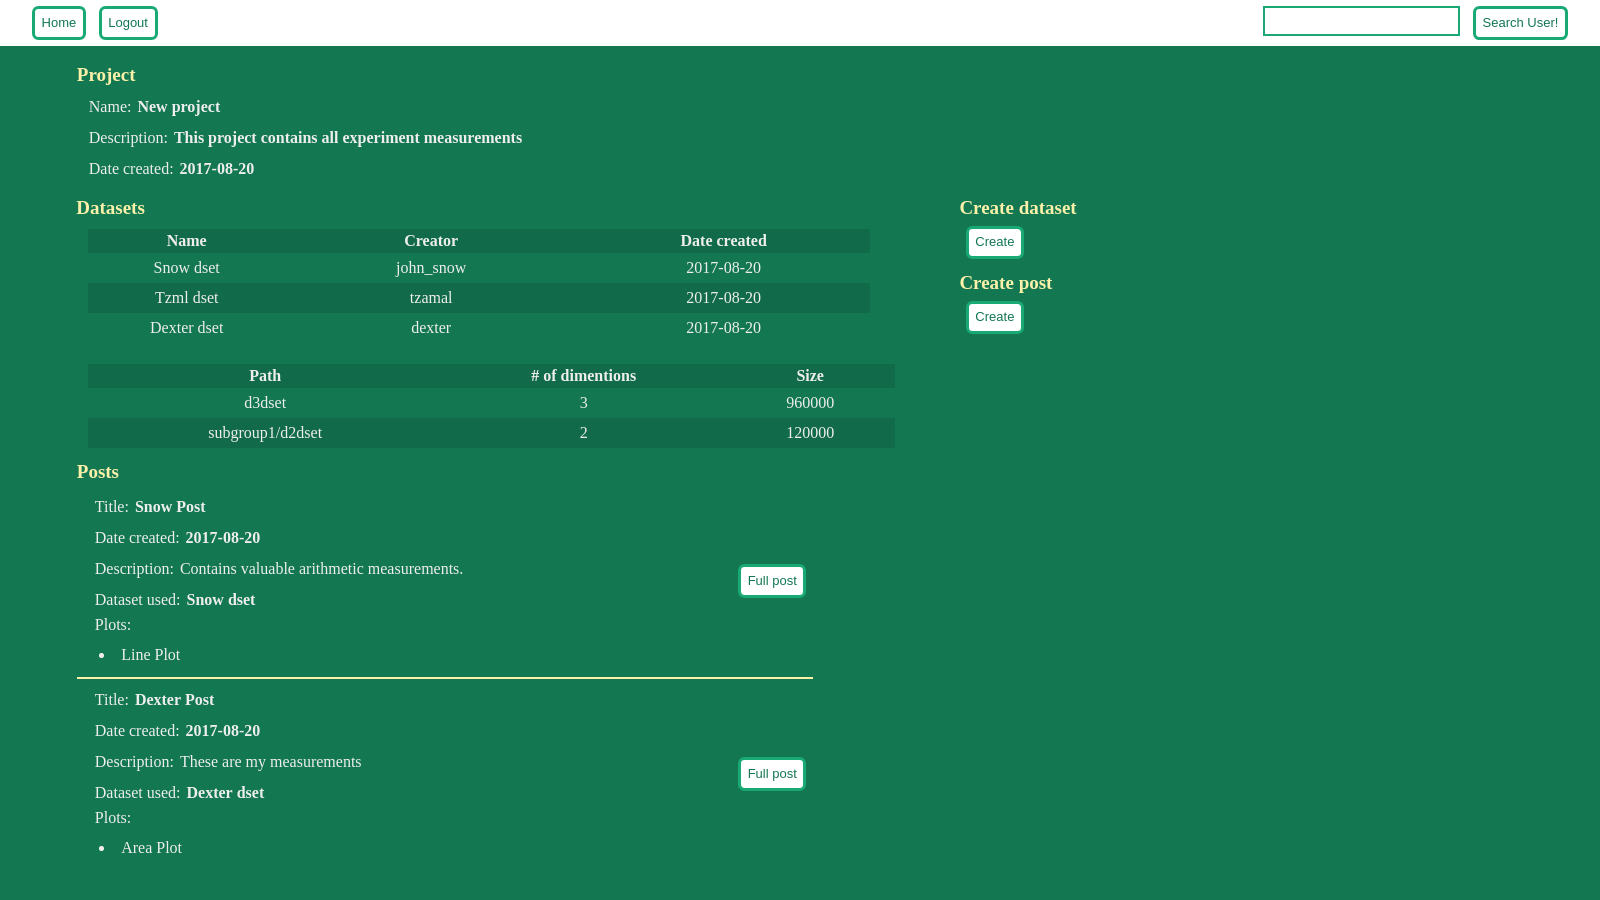
\includegraphics[width=.9\linewidth]{projectcontents.png}
  \caption{Project contents page}
\end{subfigure}
}
\caption{First pages of the application example}
\label{firstfour}
\end{figure}





\begin{figure}
\centerline
{
\begin{subfigure}{0.7\textwidth}
  \centering
  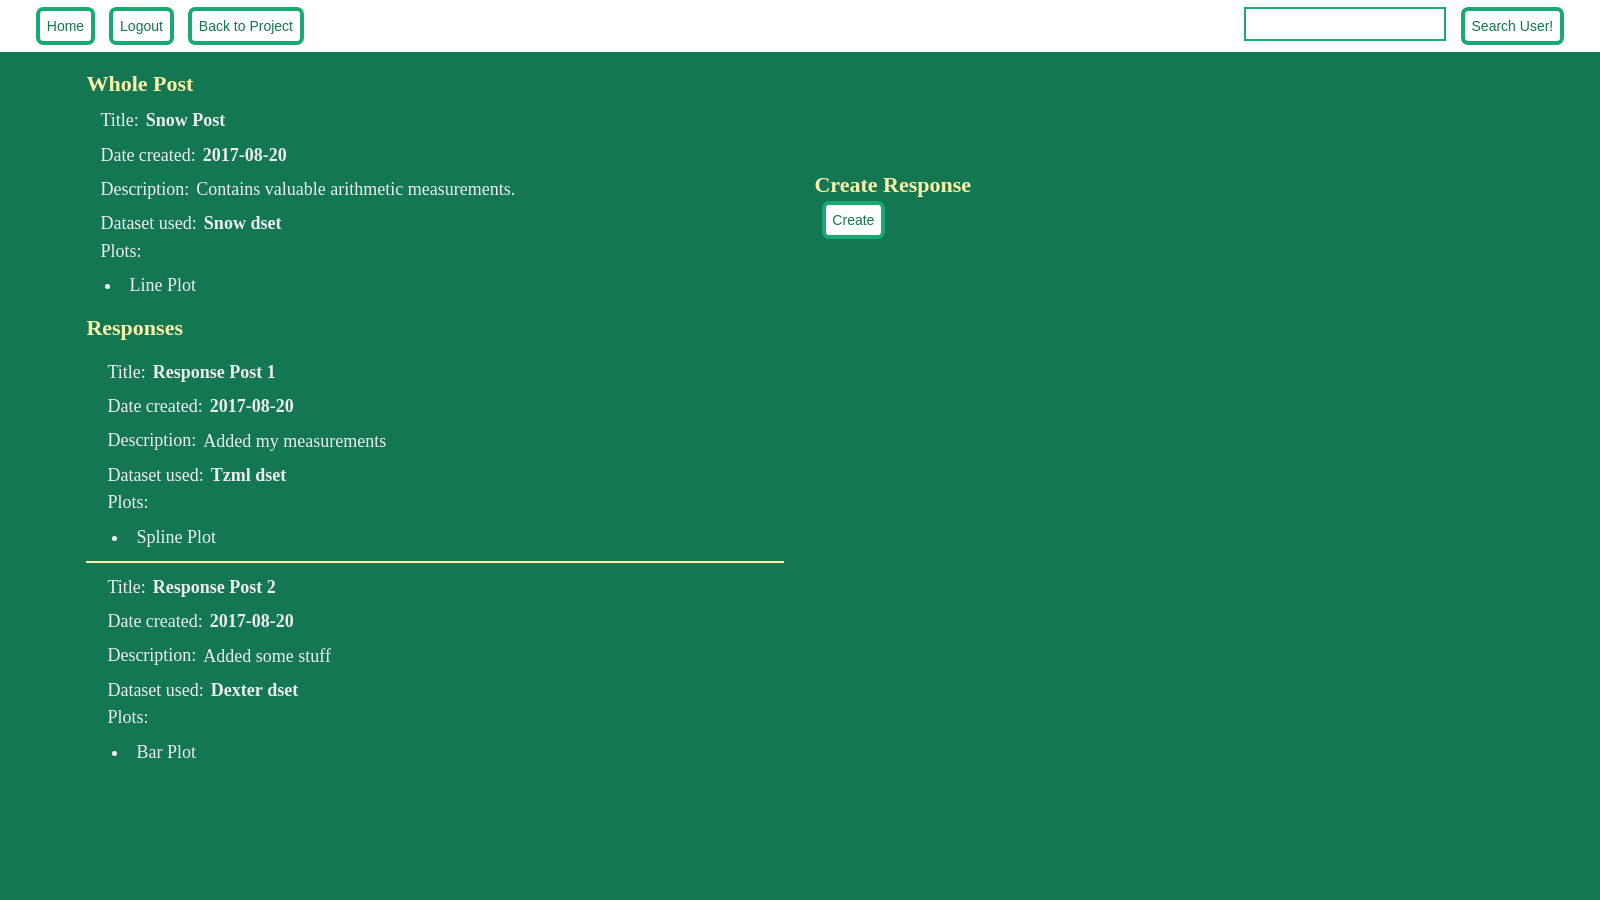
\includegraphics[width=.9\linewidth]{wholepost.png}
  \caption{Show whole post page}
\end{subfigure}%
\begin{subfigure}{0.7\textwidth}
  \centering
  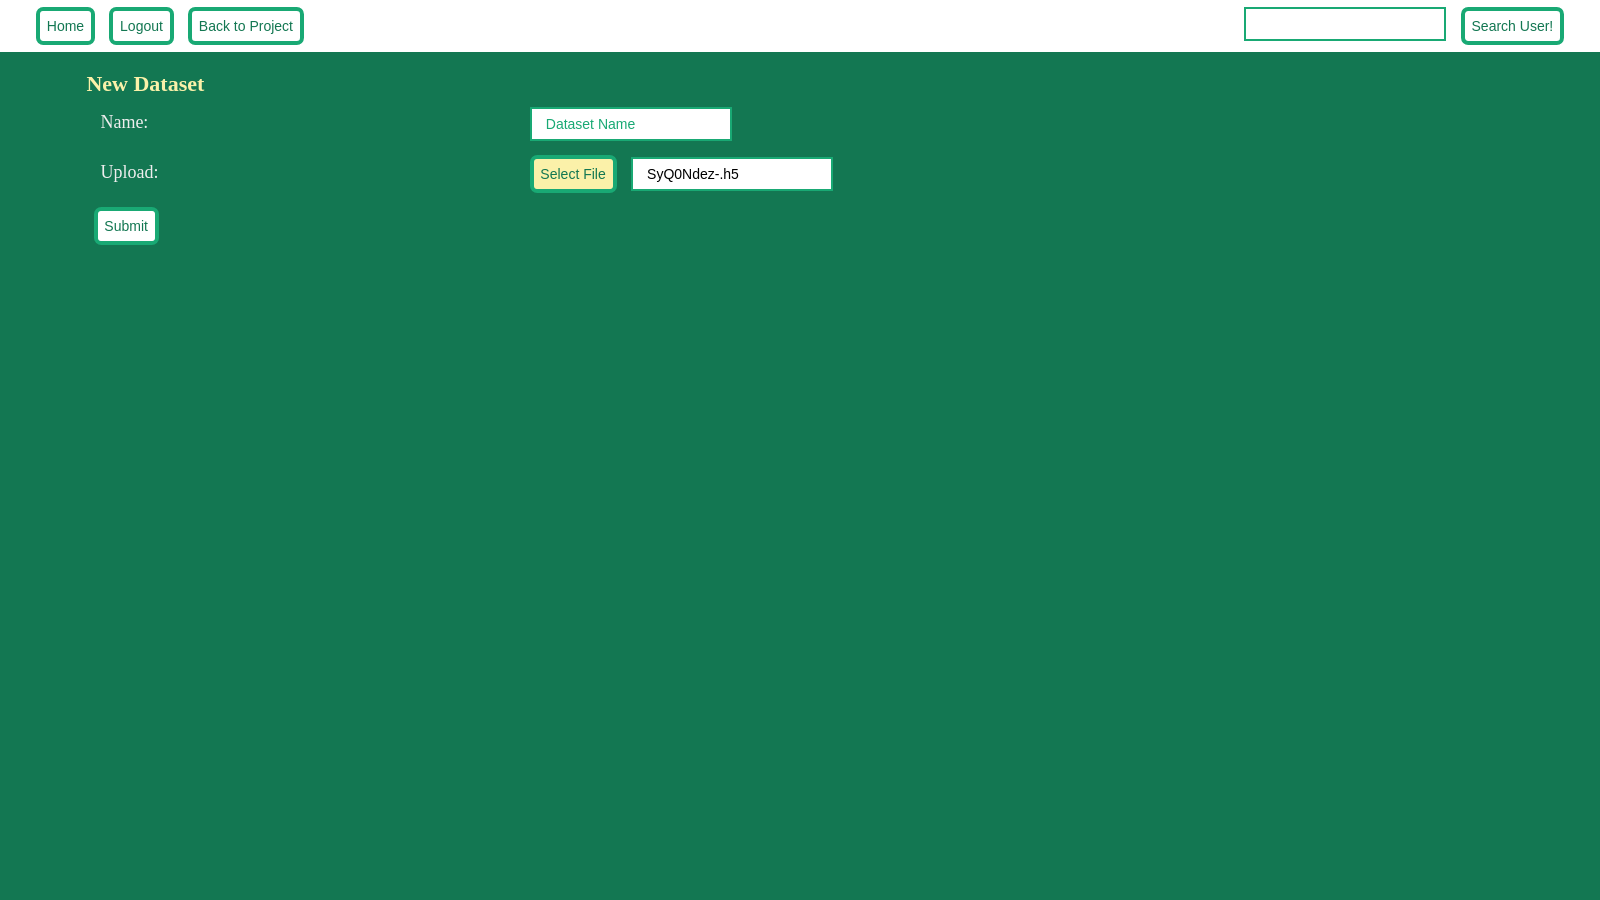
\includegraphics[width=.9\linewidth]{newdataset.png}
  \caption{Create new dataset page}
\end{subfigure}
}
\centerline
{
\begin{subfigure}{0.7\textwidth}
  \centering
  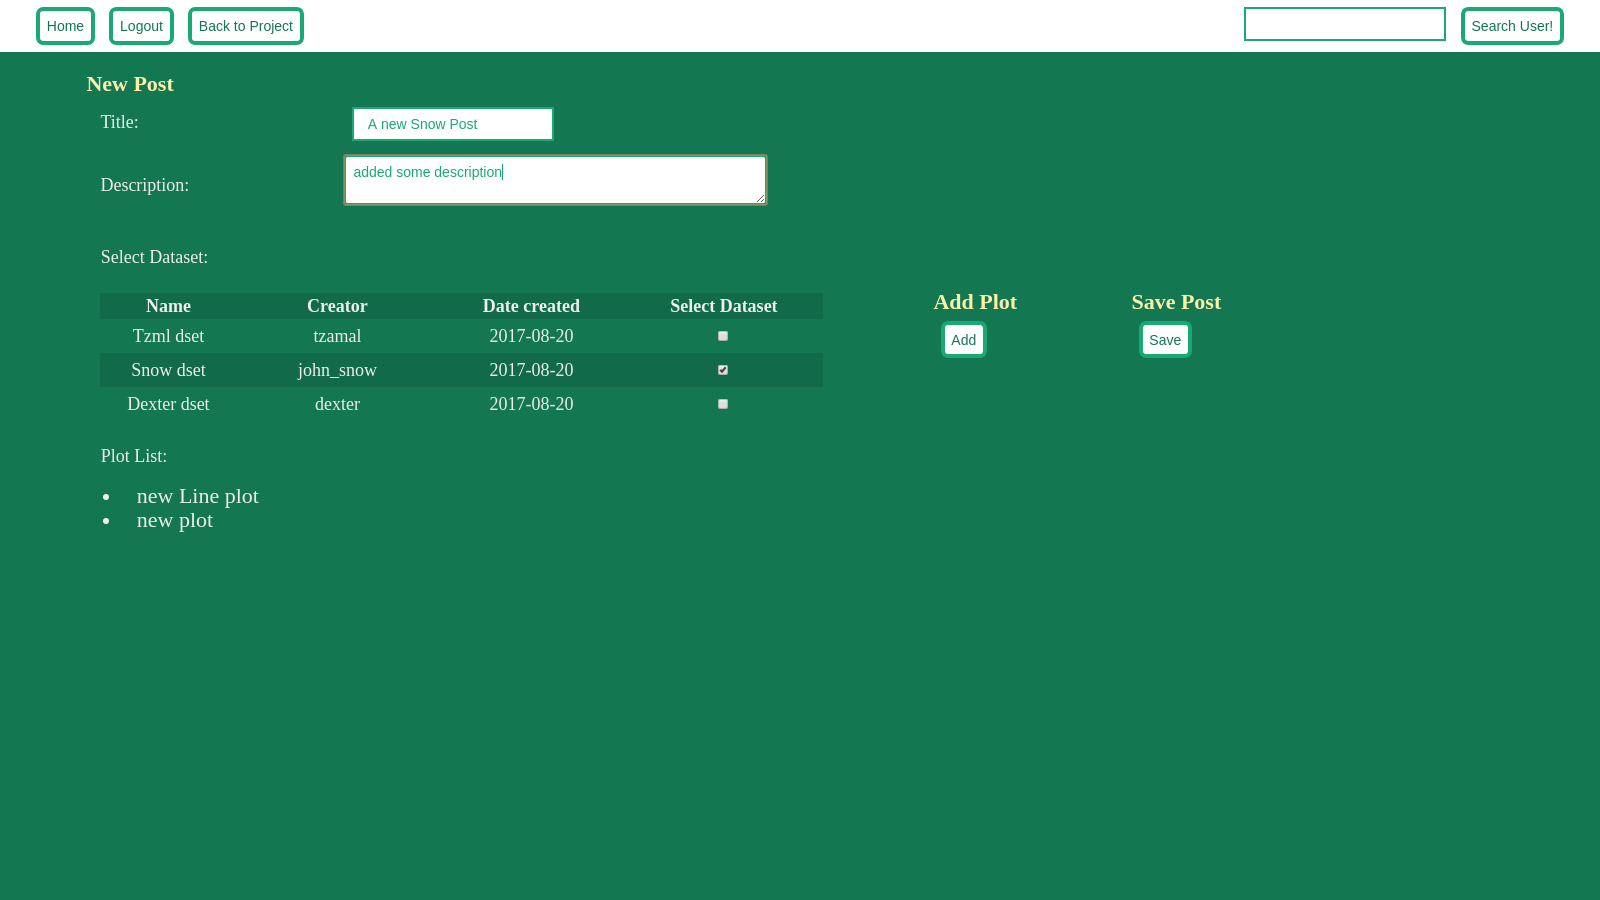
\includegraphics[width=.9\linewidth]{newpost.png}
  \caption{Create new post page}
\end{subfigure}%
\begin{subfigure}{0.7\textwidth}
  \centering
  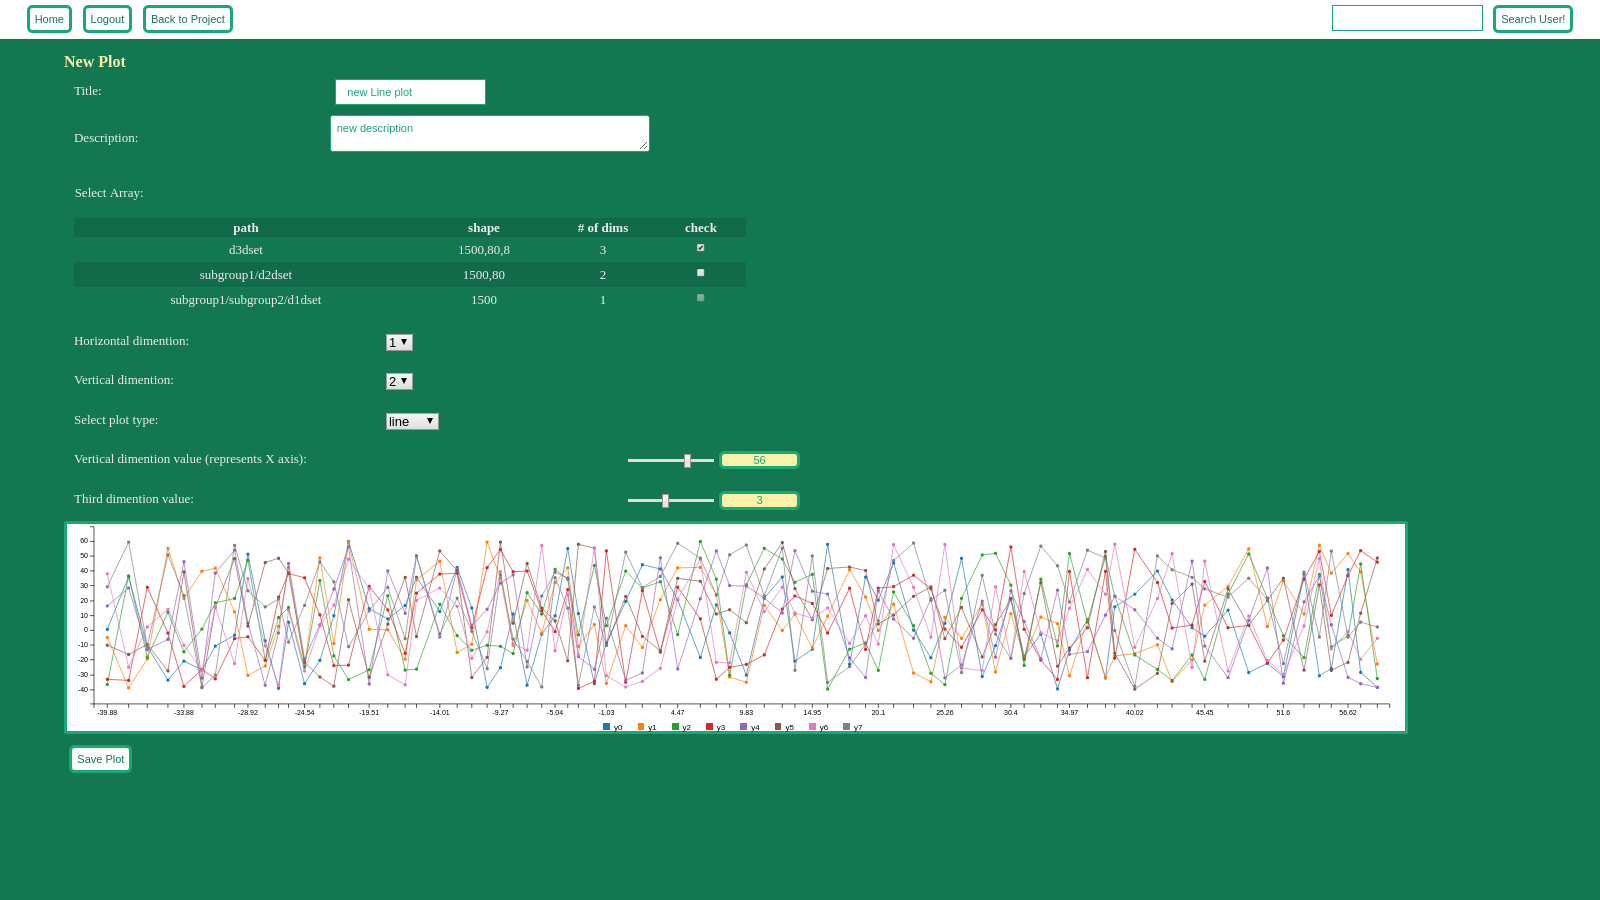
\includegraphics[width=.9\linewidth]{newplot.png}
  \caption{Create new plot page}
\end{subfigure}
}
\caption{Some more pages of the application example}
\end{figure}


\begin{figure}
\centerline
{
\begin{subfigure}{0.7\textwidth}
  \centering
  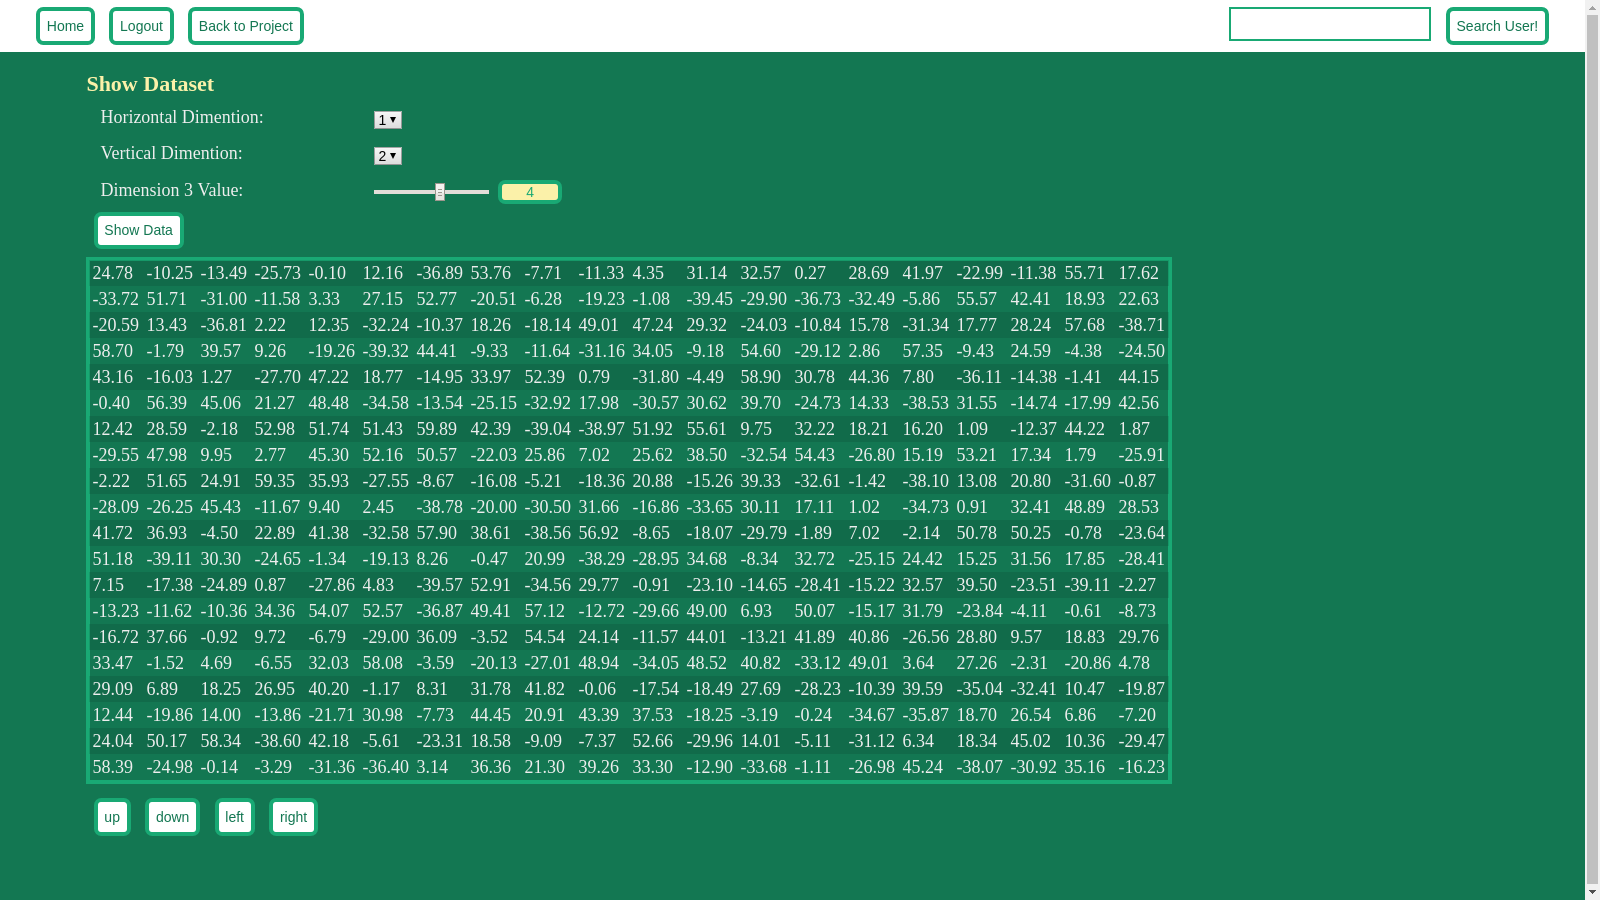
\includegraphics[width=.9\linewidth]{datasetcontents.png}
  \caption{Dataset contents page}
\end{subfigure}%
\begin{subfigure}{0.7\textwidth}
  \centering
  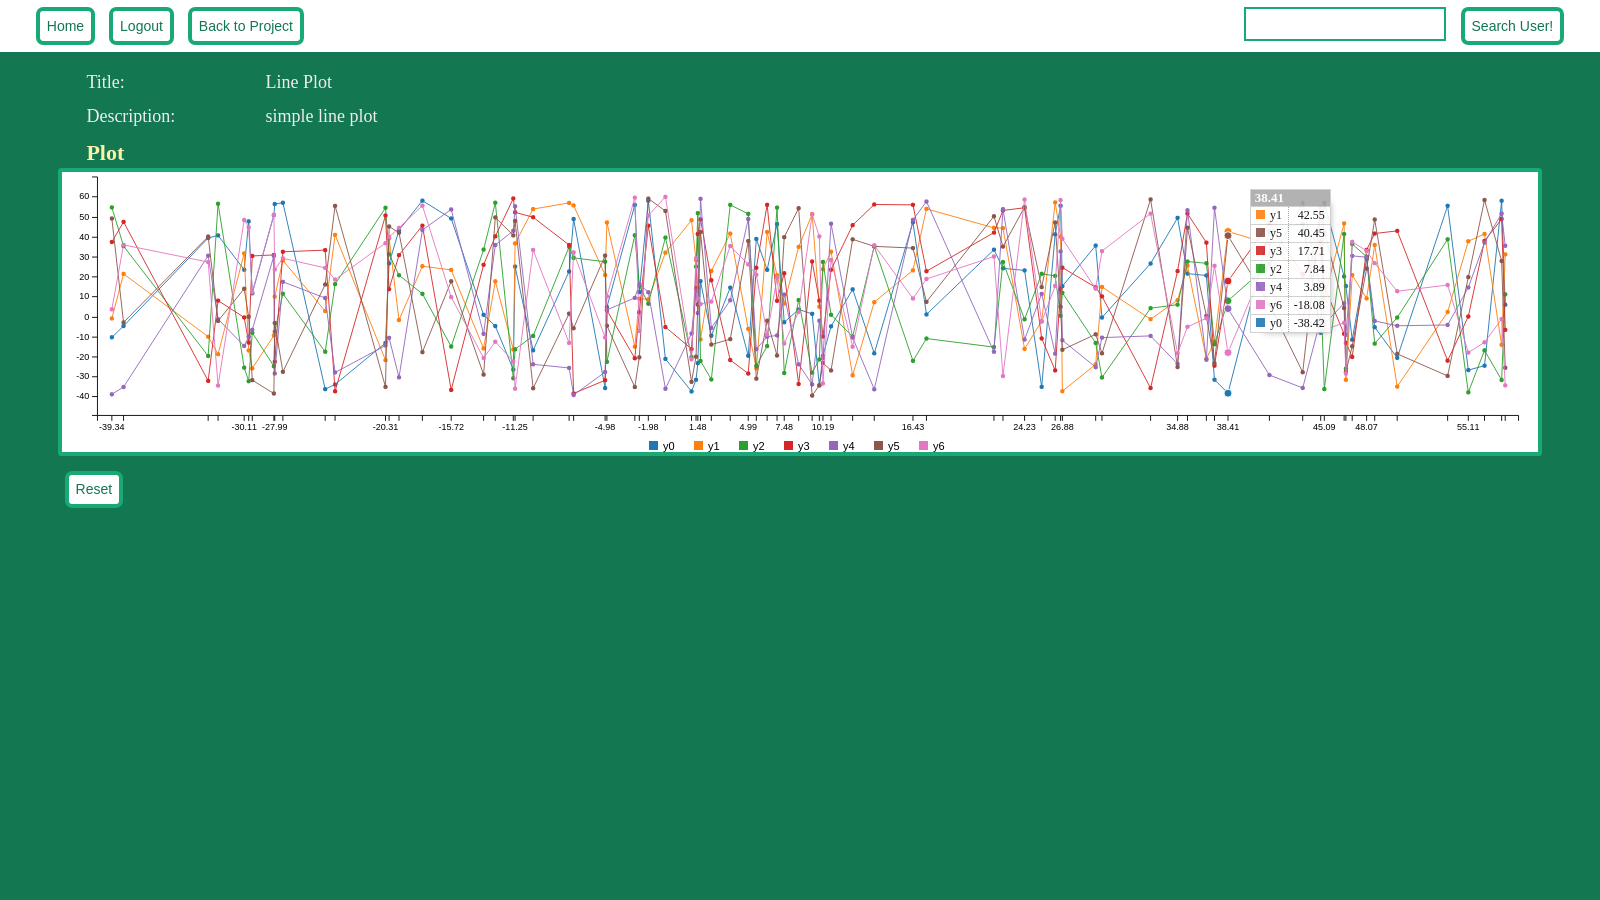
\includegraphics[width=.9\linewidth]{plotcontents.png}
  \caption{Plot contents page}
\end{subfigure}
}
\caption{Last pages presenting dataset and plot contents respectively}
\end{figure}


